\chapter{Framework design procedure}

This section outlines the methodology and design decisions in designing a complete framework that would allow for the design of a chew classifier using raw signal data from experiments where cattle were filmed while eartag signal data was recorded. This section is broken down into the following parts.

\begin{itemize}
\item Data Curation - Detailing the process of storing the large amount of binary data in an easy to access format for analysis

\item Data Annotation - Detailing the process of both building an interface to annotate the signal data with chew or non chew events and using that interface to annotate the data

\item Classifier Design - Detailing the process of designing a classifier that is based upon the annotated data
\end{itemize}

\section{Data curation}

To build training and validation sets for behaviour classification, experiments were performed in which video was recorded of two cows with sensor nodes on both the ear and halter over a span of three days. The sensor nodes logged data from accelerometer, magnometer, gyroscope, pressure, temperature and audio sensors to SD card in the Tagged Data Format (TDF). 

\subsection{Data conversion and storage}

\subsubsection{Data storage}
\label{Data storage}
The Tagged Data Format is not indexable so it was necessary to convert the data stored in this format to a format in which the data was easy to access and search through. For this purpose, the Hierarchical Data Format (HDF) was selected. HDF is a data format designed for use with large amounts of scientific data that is written once but read many times. (citation here) Additionally, mechanisms were already in place to allow for HDF files to be placed on a server and accessed remotely using a RESTful interface. 

Each individual sensor node was allocated its own HDF file, and each HDF file had a standard format and hierarchy. The format and hierarchy of the sensor node HDF files is shown in figure \ref{HDF file structure} below. The basic structure is that there is one table per sensor, with each sensor being a physical chip on the board. Each table contained rows containing the UTC time the sensor reading was taken and the corresponding sensor measurement readings. Because of the way in which the sampling from each sensor works in the sensor node, this allows sensor readings that share sample times to be written into the same row.  

\begin{verbbox}
  - <Deployment name> 
    - Data
        - <Eartag name 1>
            + <Sensor Name 1>
            + <Sensor Name 2>

        - <Eartag name 2>
            + <Sensor Name 1>
            + <Sensor Name 2>
    - TDF
\end{verbbox}
\begin{figure}[ht!]
  \centering
  \theverbbox
  \caption{HDF file structure}
\end{figure}

The elements marked with a \texttt{+} are tables while the elements marked with \texttt{-} are groups, which assist in organising the structure. Typically, for the experiments that took place there were five sensor tables; pressure/temperature, audio, accelerometer, magnetometer and a reset counter. 

The structure of a sensor table with N measurements/sensors is presented below in figure \ref{HDF table structure}. Each table had rows of sensor readings. For example, the audio sensor had two columns, a time column and a sample column. On the other hand, the accelerometer table had four columns; a time column and a column for each of the x, y and z accelormeter readings. \\

\begin{verbbox}
Time | Sensor1 Measurement | .. | Sensor N Measurement 
\end{verbbox}
\begin{figure}[ht!]
  \centering
  \theverbbox
  \caption{HDF table structure}
\end{figure}

\subsubsection{Data conversion}
To convert the TDF data to HDF data, a python command line utility was written that made use of the python library, PyTables which exposes the HDF5 library to python bindings. The python script was written to extract and then parse the binary, TDF data into memory before writing it all out to a specified HDF file. A full code listing of the completed command line utility, \texttt{sd2hdf} can be found in appendix \ref{appendix - sd2hdf}. 

Audio was sampled at approximately 24 kHz and 12 bits. However, to save space when saving the audio samples to SD card, audio samples were saved in chunks. This meant that only the sample time of the first audio sample in the chunk was known. To find the precise sampling period so that it was possible to record an accurate time for each individual audio sample, the time between chunks had to be used.  

Initially, the size of the HDF files were over 100GB. To reduce the size of these files, the python script was modified to use BLOSC compression when writing to the HDF files. This reduced the size of the HDF files by approximately a factor of 10.

After the script was run and HDF files were produced, these were placed on a server which allowed the data to be accessed remotely over a RESTful JSON interface. This allowed for downloading data within certain time periods, from certain sensors and from certain nodes. 

\subsubsection{Data extraction}
\label{extraction}
The RESTful interface made it possible to easily extract JSON formatted sensor data using HTTP requests. The following URL is an example of a request for sensor data over this interface. 

\url{http://livestock.sensornets.csiro.au/data/v1/network/bigridge4/platform/eartag732/sensor/LSM303DLHC\_MAG/observations?\&limit=22000\&start=2013-12-02T23:15:00\&end=2013-12-02T23:15:01} 

This request will get a JSON response that contains LSM303DLHC\_MAG sensor data (which is magnometer sensor data) from an eartag named eartag732 for the Big Ridge 4 experiment between the start and end dates listed in the query. 

The structure of the returned JSON is shown below in figure \ref{JSON structure}. For brevity, only the first two observations in the JSON file are shown. Each successive observation is of the form of the two shown. 

\begin{verbbox}
{
    "query_time": "0:00:00.813353",

    "observations": [
            {
                "magz": 0.5625,
                "magy": 0.29555556178092957,
                "magx": -0.05111110955476761,
                "utc": "2013-12-03T06:09:33.580169"
            },
            {
                "magz": 0.5625,
                "magy": 0.30444443225860596,
                "magx": -0.046666666865348816,
                "utc": "2013-12-03T06:09:33.515869"
            },
        ]

    "title": "showing 100 from 431999 observations"
}
\end{verbbox}
\begin{figure}[ht!]
  \centering
  \theverbbox
  \caption{JSON structure}
\end{figure}

The important part of the returned JSON is the data in the \texttt{observations} field. This field is a list of dictionaries where each dictionary contains measurement from the sensor along with the corresponding time that measurements were taken. In this case, because the magnometer used is triaxial, there are three measurements; \texttt{magx}, \texttt{magy}, \texttt{magz}. The time of sample is in the \texttt{utc} field which is stored as a UTC time. For other sensors, such as the audio sensor, there are not as many measurements per data point. 

\subsection{Data coverage plotting}

In the two experiments that were performed, there were some reliability issues for the sensor nodes that were used. In some cases, some sensor nodes stopped working completely and needed to be replaced while in other cases certain sensors on the sensor nodes did not record data for some periods of time. In addition to this, video was only recorded for a very small amount of time compared to the amount of sensor node data that was recorded. 

In order to develop a training set based on the recorded data it was neccesary to find time periods where there was complete sensor data coverage as well as corresponding video coverage. To do this a python script was written that iterated through the signal data. The script found the time difference between adjacent data samples and if the difference was larger than a threshold recorded that period of time between samples as a gap. This threshold was different for each signal as each signal had different sampling rates. 

After the gaps were found then it was possible to plot the coverage of different signal nodes over the experiment time frame. An example of this is shown in figure \ref{coverage_plot}. The solid line in the figure represents continous signal coverage (no gaps in the data) whereas a gap in the line signifies there are no samples captured for that time period. 

\begin{figure}[ht!]
\begin{center}
\leavevmode
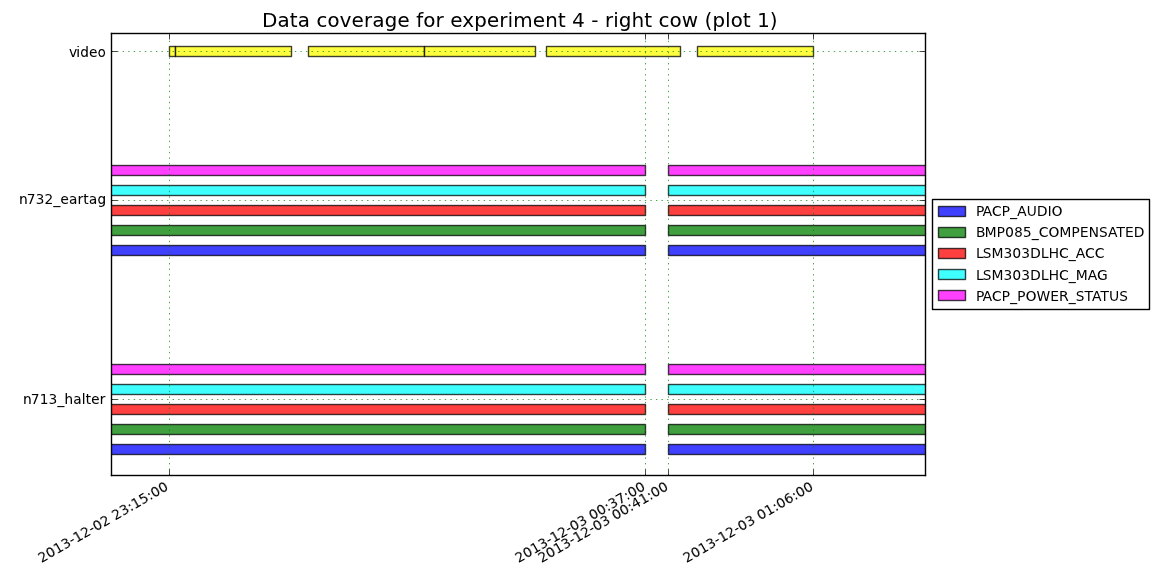
\includegraphics[width=0.8\textwidth]{images/experiment4_coverage_zoomed.png}
\end{center}
\caption{Data coverage of cow in plot 1 in experiment 4}
\label{exp4overall}
\end{figure}

Using this figures it was then possible to quickly locate periods where there both signal data and video recordings existed. These periods were then able to be annotated and used for classifier design. 


\section{Data annotation}

In order to create training and test sets so that an algorithm for classification of cow behaviour could be built it was necessary to annotate the recorded signals from the experiments performed. This meant manually looking the recorded data signals, listening to the recorded audio from the sensor nodes and watching the associated video to find individual chew events. To assist with this process, an annotation interface was designed. 

\subsection{Annotation storage}

Annotations were stored in the HDF system as described in section \ref{Data storage}. Annotations were considered a type of sensor so that each eartag device would have its own annotation table in the data system. The structure for the annotation table followed from the structure of the other sensor tables and is shown below in figure \ref{annotation table structure}.

\begin{verbbox}
Time | Event | Duration | Annotator | Confidence | Reference
\end{verbbox}
\begin{figure}[ht!]
  \centering
  \theverbbox
  \caption{HDF table structure}
\end{figure}

The purpose of each field and the format that the data is stored in is discussed in the list below.

\begin{itemize}
\item Time: The start time of the event as an UTC time.

\item Event: A string of what the event was, for example 'chew' or `not chew'.

\item Duation: The length of the event as an integer in microsecond.

\item Annotator: Describes the annotation method used to make the annotation. This could either be a person's name in the case of a manual annotation or, in the case of an automated classifier, the type of automated classifer that made the annotation.

\item Confidence: The confidence level that the annotator had when annotating as an integer percentage

\item Reference: A string describing was used to make the annotation. For a human annotator this could be a particular bit of data or a video file. 
\end{itemize}

Because the annotation was stored in the same way as the sensor data, it could be accessed in the same way through the RESTful JSON interface that was previously described in section \ref{extraction}. 

\subsection{Annotation submission}
As the data from the annotations was generated in a different way to the sensor data, a different method had to be devised to submit annotations to the HDF system. To do this, the \texttt{annotation\_push.py} command line utility was written. A full code listing of this utility can be found in appendix \label{appendixannotationpush}.

The \texttt{annotation\_push.py} file was written so that it could be used as a library with other python code. This allowed the annotation interface (described in the next section) to use it for submitting annotations. 

The script works by formatting the annotation data (the fields for the table as well as information about what node and deployment the annotation corresponds to) into a dictionary which it then converts to JSON before submitting to an ingestion web-service. The ingestion web-service takes the JSON and enters the information into the corresponding table. 

\subsection{Annotation interface}


\subsubsection{Annotation interface launcher}

To streamline the process of selecting the data to be annotated in the annotation interface, a launcher was developed using the Graphical User Interface (GUI) library Wx \cite{rappin2006wxpython}. The launcher GUI is shown below in figure \ref{launcherpic}. It allows the user to choose any combination of sensors from any avaliable sensor node and deployment. 

\begin{figure}[ht!]
\begin{center}
\leavevmode
\includegraphics[width=0.5\textwidth]{images/annotationlauncher.png}
\end{center}
\caption{Annotation interface launcher GUI}
\label{launcherpic}
\end{figure}

This launcher dynamically loaded all sections from the RESTful service. It also allows the user the choice of displaying or not displaying the previously annotated sections of the selected data. 

\subsubsection{Annotation interface application}

In designing the interface for annotation it was important to allow a view of each of the different signals captured. It was also important to do this modularly so that the interface could be reused as a tool to annotate different sorts of data.

Figure \ref{annotation_interface_design} shows the initial design of the interface. The interface shows the signal data from a number of different sensors. It allows a user to select a period of signal data (the red box shows the currently selected period), choose an annotation category (in this case, either 'chew' or 'not chew') and then submit the annotation. In addition, the interface also shows the time period currently selected and allows a user to play the audio from the selected period. 

\begin{figure}[ht!]
\begin{center}
\leavevmode
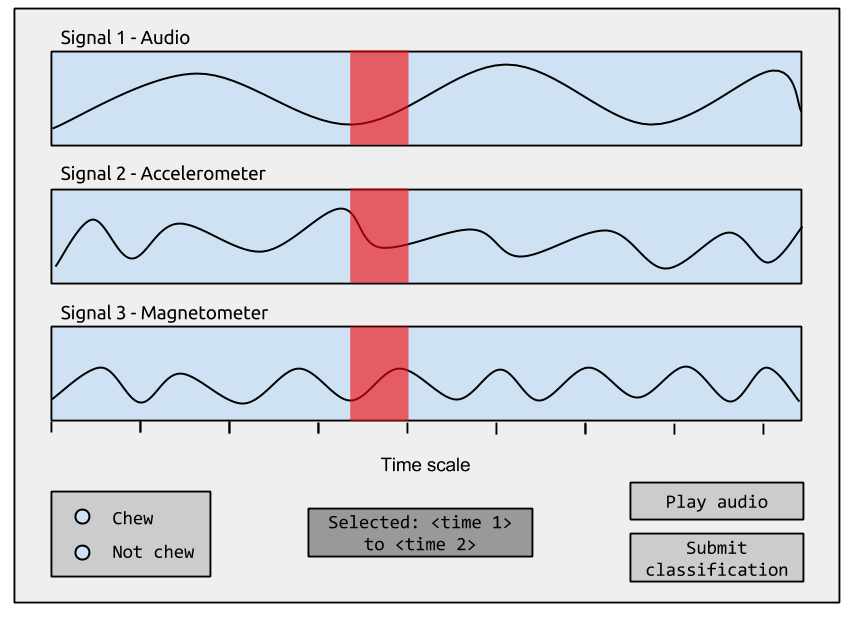
\includegraphics[width=0.8\textwidth]{images/annotation_interface_design.png}
\end{center}
\caption{Annotation interface design}
\label{annotationinterfacedesign}
\end{figure}

To mesh well with the existing code base and for quick prototyping and cross compatibility, the annotation graphical user interface was written using python. Because much of the interface would involve displaying signal data in the way of plots, the matplotlib library was used to assist with the creation of the interface. As well as containing the tools to allow for creating data plots the matplotlib library contains widgets (for example, buttons or selector items) that can be used to make plots more dynamic. 

The inbuilt matplotlib SpanSelector widget was used in the interface so that a very simple click and drag selection process could be used to select sections of data. This allows a user to select a section of data. When done, the start and end time of the selected period is displayed in the interface. The interface also contains a selector widget that allows the user to choose between different event categories to annotate, specifically either 'chew' or `not chew'. Finally, the interface contains a button that allows the user to submit the annotation. A submitted annotation is stored in the HDF data structure discussed in section \ref{data curation - annotation}. 

The interface also contains functionality to play a selected period of audio. This was enabled by the \texttt{scikits.audiolab} python library \cite{Cournapeau}. Because of the limitations of this library and the way that it interfaces with the Mac Core Audio library, this only allowed for audio to be played at the standard sampling rate of 44.1 kHz. Fortunately, the audio recorded as part of the experiments that were used was at approximately 22 kHz so it was possible to oversample the audio at double the rate in order to play it. In this case, as the audio is only used to find the start and end of an annotation period, the precise playback frequency is not of great importance. 

The audio playing functionality is implemented in the interface as a play button that plays the audio associated with the currently selected time period. A user of the annotation interface is then able to select a node, a time period and a range of sensors to be displayed in the interface. Events can then be found within that time period and the audio can be used to precisely find the start and end times. 

A annotated version of the finished interface is shown in figure \ref{annotationinterface}. This image shows a previously annotated one minute section of data. The data is from three different sensors - an acceloremeter, a magnetometer and a microphone. The sections of the data highlighted red indicate that that section of data was annotated as a chew event while the blue sections indicate that that section of data was annotated as an other event. 

\begin{figure}[ht!]
\begin{center}
\leavevmode
\includegraphics[width=0.9\textwidth]{images/annotation_interface_annotated.png}
\end{center}
\caption{Finished version of the annotation interface}
\label{annotationinterface}
\end{figure}

\subsection{Annotation set building}

Events were classified into two different classification categories when building the training set. These modes were a 'chew' mode and a 'not chew' mode. It was important to build the classification set to contain both of these events so that a classifier would know how to classify both. 

It was also important to build the training set such that the events selected roughly represented the all variations in the two modes. This meant ensuring that events were picked from a range of different times over a range of different conditions.

To find time periods to classify, the videos of the experiment were used. These videos helped to broadly classify a particular cow's behaviour over a time period but were not very helpful in finding the exact time periods of events. As mentioned in the previous section, it was necessary to use the audio and other signal data to precisely select the start and end of events. 

\section{Classifier design}

The design of the classifier comprised of two parts; deciding on an algorithm to use and then investigating the best way to design or train it and then implementing methods to validate and test the accuracy of the classifer.  

\subsection{Selection of algorithm}

In choosing an algorithm to use to classify the signal data into chew or not chew categories, an investigation was performed into different types of algorithms and paradigms. The two main paradigms that were examined were algorithms that followed a simple thresholding/signal processing approach and supervised machine learning algorithms. 

The machine learning approach was found to be better in its ability to take full advantage of the high dimensionality of the signal data. A machine learning algorithm is able to take advantage of trends and patterns in the data that a human may not be able to directly identify. This in contrast to signal processing approach where trends in the data need to be manually found. The framework was then written to be able to use any machine learning algorithm. The paradigm for most machine learning algorithms is similar as detailed in section \label{classifierframework}.

For prototyping, the SVM algorithm was chosen for the classifier. As well as being fast to converge to a result, the SVM algorithm has also be extensively studied and used in practice so there are many free and open source software libraries that can be used to implement the algorithm. In addition, the SVM algorithm was also appealing as it has shown to be feasible to run on embedded and resource constrained hardware. 

\subsection{Selection of classifier prototyping software}

Although the classifier would eventually run on embedded hardware and need to be written in the C programming language, the classifier was designed and prototyped using Python. This allowed for easy combination with the rest of the data extraction and storage framework. 

Python also has the advantage of being a mature development environment, particularly for scientific computing. Libraries such as numpy \cite{numpy}, scipy \cite{scipy} and matplotlib \cite{matplotlib} enabled easy analysis and quick prototyping. 

Writing the classifier training and validation parts of the framework in python also enabled the framework to fit together better, allowing for a complete work flow in python. This not only minimises the need for extra development software but also simplifies the process of writing extensions to the framework in the future. 

The scikits.learn package was used for most of the machine learning algorithm design process. As well as having a full implementation of the SVM algorithm, it also includes numerous other useful utilities for such tasks as normalisation and training/test set partitioning. 

\subsection{Classifier framework}
\label{classifierframework}

The process to build a robust classifier consisted of:

\begin{enumerate}
\item Retrieving the annotations and annotated data

\item Randomly splitting the complete data set into training and validation sets

\item Extracting features from the data

\item Statistically normalising the features

\item Using the features to train a SVM classifier

\item Validating and assessing the accuracy of the classifier using the validation set
\end{enumerate}

This process is discussed in more detail below. 

\subsection{Selection of features}
In order to design a robust algorithm that could classify signal data into categories, features of the data need to first be extracted from the data. Features can be the result of running simple functions over a small dataset, such as a min, max or mean operation but can also be more complicated functions such as a Fourier transform. 

The part of the framework used for training a classifier, contained in the file \texttt{train.py}, was written modularly to allow for any features to be used. This is shown in the code snippet below. Any function name name be put into the list of feature function. The training code will use all the function in this list to extract the features from the annotated data. 

\begin{verbatim}
time_invariant = [np.mean, np.std, np.min, np.max, ff.half_window_difference]
\end{verbatim}

These methods all take data in a list or vector structure and perform an operation on the data, giving back a single number. However, the framework allows for methods which can take data in a list or vector structure and return data in a list or vector structure. This could be useful for more advanced features. 

\subsection{Feature normalisation and scaling}
In order for the features fed to a machine learning classifier were of the same average magnitude and deviation, the features were first normlalised and scaled. The Scikits-learn feature normalisation functionality was used for this. This allowed a scaler object to be saved, so that the test data could be scaled and normalised in the same way that the training data was. 

\subsection{Classifier training}
Once the features were extracted from the training data they were used to train a classifier. Using Scikits-learn, this was as simple as calling the \texttt{fit} method on a classifier model. This function fits the model to the data. 

The classifier and scaler could then be saved as pipeline. The pipeline is a feature of Scikits-learn that allows method calls to be put together into a struture. This structure can be saved and new data can be passed to it. 

The following code snippet shows the process of training a model. In this case a SVM is being trained but any classifier could be trained in the same way.

\begin{verbatim}
def train_svm(positive_data, negative_data):
    pos_features = datatools.get_data_features(positive_data, sensors, feature_fns)
    neg_features = datatools.get_data_features(negative_data, sensors, feature_fns)
    
    X = np.array(pos_features + neg_features)
    y = np.array([1]*len(pos_features) + [0]*len(neg_features))
    
    X_train, X_test, y_train, y_test = train_test_split(X, y, test_size=0.3)
    
    scaler = preprocessing.StandardScaler().fit(X_train)
    X_train = scaler.transform(X_train)
    
    clf = svm.SVC(class_weight='auto')
    clf.fit(X_train, y_train) 
    
    pipeline = Pipeline([('scaler', scaler), ('svc', clf)])
\end{verbatim}


This code first extracts features from the annotated data using the \texttt{feature\_fns} list previously described. An \textit{X} matrix is then formed which contains columns of features from each event. The \textit{y} vector contains the corresponding classification for each event. In this case, the positive event data is labelled with \texttt{1} and the negative event data is labelled with \texttt{0}.

The set is then split into a training and test set, scaled and then the data is used to fit a SVM model. The SVM model as well as the scaler can then be saved into a pipeline for use with new data later.  

\section{Classifier evaluation}
In order to properly evaluate the performance of a potential classifier, a framework to evaluate the classifier needed to be built. This classifier would be tested on previously annotated datasets that were not used in the classifier design/training phases. 

\subsection{Partitioning the annotation set}
To partition the previous annotated data set into both a set to train the classifier and a set to test the classifier, the \texttt{train\_test\_split} function was used from the \texttt{scikits.learn} toolkit. This function takes a X matrix containing columns of features and a Y vector containing the corresponding annotation for each column. 

The function can then randomly split X and Y into a training and testing set. This ensures that there is diversity across both sets. The size of each set can also be controlled by passing a parameter to the function. 

This splitting of the annotated set was performed after the extraction of the features from the data but before the features were scaled. This is so the scaler would be created only from the training data so that it is not biased by data that was not used to train it. 

\subsection{Confidence level estimation}
As it is possible to seed the random number generator the \texttt{train\_test\_split} method uses to split the data set, this feature was used to estimate a confidence level of a classifier.

By using a number of different seeds for the \texttt{train\_test\_split} method, classifiers would be trained and tested on different parts of the data. Doing this enough times allowed for an estimation of the range of accuracy of the classifier. This helped to ensure the classifier was robust. 

\subsection{Testing on non annotated data}
The previous methods for validation of the classifier tested on data that was already annotated. When designing a classifier it would still be valuable to validate its performance on sections of non annotated data. It would also be valuable to validate classifiers across data sets in the same way as they would be used when running on a device in the field. 

The basic premise of this method of testing can be thought of as having a window of a fixed time period that is moved across the data. At each position of the window, a new classification is made. 

This method of validation is implemented in \texttt{predictor.py}. The following code snippet demonstrates the basic block of the code.

\begin{verbatim}
while start < end:
    #get the end of the current window
    end_window = start + window_length
    
    #extract the window data from the data
    period_data = extract_from_data(data[0], start, end_window)
    
    #get the required features
    features = datatools.get_data_features([period_data], sensors, feature_fns)
    
    #get the prediction result from the features
    prediction = get_prediction(features)[0]
    pos_preds += prediction
    predictions.append((start, end_window, prediction))
        
    start += us_step
\end{verbatim}

This code moves the window of \texttt{window\_length} along at increments of \texttt{us\_step}, making a prediction using the data in the window at each step. The list of predictions is then saved and can be displayed in the annotation interface by choosing a prediction file in the launcher part of the interface. An example output when loading in a prediction file is shown in figure \ref{interfaceprediction}.

In this case, as before the red and blue highlighted sections represent the chew or not chew events as before. The black line is the classification at each position of the window, with a high value representing a chew event and a low value representing a non chew event. The value of classification at each point is the classification for the preceeding window so the classifier value is approximately one window length behind the manual annotation, which explains the mismatch.

\begin{figure}[ht!]
\begin{center}
\leavevmode
\includegraphics[width=0.9\textwidth]{images/annotation_interface_predictions.png}
\end{center}
\caption{Annotation interface with predictions}
\label{interfaceprediction}
\end{figure}

%aeropress espresso

%\subsection{Feature scoring (maybe this is better in the section before though)}


%% maybe useful stuff:
%% paper with stuff about ML algos for emebedded systems %%http://nesl.ee.ucla.edu/courses/ee202a/shared/samples/projects/2008f/Adam_Stoelting.pdf%%